\documentclass{beamer}
\usepackage{graphicx}

% Choose how your presentation looks.
%
% For more themes, color themes and font themes, see:
% http://deic.uab.es/~iblanes/beamer_gallery/index_by_theme.html
%
\mode<presentation>
{
  \usetheme{default}      % or try Darmstadt, Madrid, Warsaw, ...
  \usecolortheme{default} % or try albatross, beaver, crane, ...
  \usefonttheme{default}  % or try serif, structurebold, ...
  \setbeamertemplate{navigation symbols}{}
  \setbeamertemplate{caption}[numbered]
} 

\usepackage[english]{babel}
\usepackage[utf8x]{inputenc}

\title[Simultaneous Evolution of Morphology and Locomotion of Soft Robots by Novelty Search]{Simultaneous Evolution of Morphology and Locomotion of Soft Robots by Novelty Search}
\author{Georgios Methenitis}
\institute{University of Amsterdam}
\date{\today}

\begin{document}

\begin{frame}
  \titlepage
\end{frame}

% Uncomment these lines for an automatically generated outline.
%\begin{frame}{Outline}
%  \tableofcontents
%\end{frame}

\section{Introduction}
\begin{frame}{Introduction}
\begin{block}{Soft Robots}
\begin{itemize}
\item Inspired by nature
\item Completely soft bodies
\item Capable of developing new kinds of locomotion
\end{itemize}
\end{block}
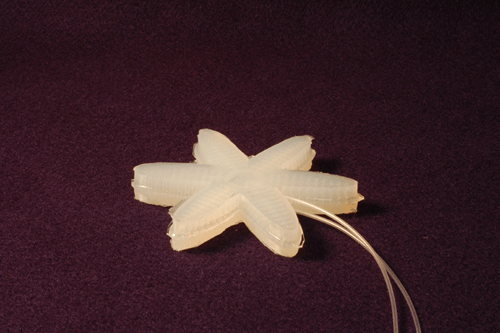
\includegraphics[width=0.3\textwidth,height=0.25\textheight]{figures/soft_robotics_figure.png}\	
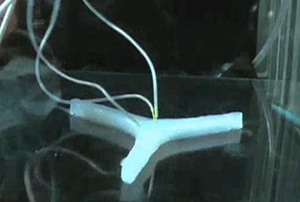
\includegraphics[width=0.3\textwidth,height=0.25\textheight]{figures/ExplodingRobot.jpg}\	
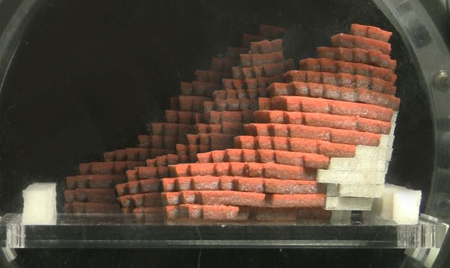
\includegraphics[width=0.3\textwidth,height=0.25\textheight]{figures/hillerPressureChamber.png}\\
\vspace{0.3cm}
Soft robots can be actuated through air pressure tubes, environmental changes ( temperature, pressure ), even explosions.
\end{frame}

\begin{frame}{Related Material}
\end{frame}

\begin{frame}{Related Work}
\end{frame}


\end{document}